% !TEX program = xelatex
\documentclass[11pt]{article}
\usepackage{fontspec}
\usepackage{xeCJK}
\usepackage[margin=1in]{geometry}
\usepackage{amsmath}
\usepackage{amsthm}
\usepackage{graphicx}
\usepackage{tikz-cd}
\usepackage{multicol}
\usepackage{titling}
\usepackage{setspace}
\usepackage{float}
\usepackage{subcaption}
\newtheorem{theorem}{Theorem}

% Bigger & bolder title
\pretitle{\begin{center}\LARGE\bfseries}
\posttitle{\par\end{center}\vskip 0.5em}
\predate{\begin{center}}
\postdate{\end{center}}
\setlength{\droptitle}{-6em}

% Paragraph style (old)
% \setlength{\parindent}{0pt}
% \setlength{\parskip}{0.4\baselineskip}
% Paragraph style (new)
% \setlength{\parindent}{2em}
% \setlength{\parskip}{0pt}
% \setstretch{0.96}


\begin{document}

\title{Notes on Information Theory}
\author{}
\date{}
\maketitle


\begin{quote}
{\Large
  The fundamental problem of communication is that of reproducing at one point either exactly or approximately a message selected at another point.
  \begin{flushright}
    --- Claude Shannon, 1948
  \end{flushright}
}
\end{quote}

\tableofcontents
\newpage

\clearpage
\section{System Approach in Communication}

\begin{figure}[H]
  \centering
  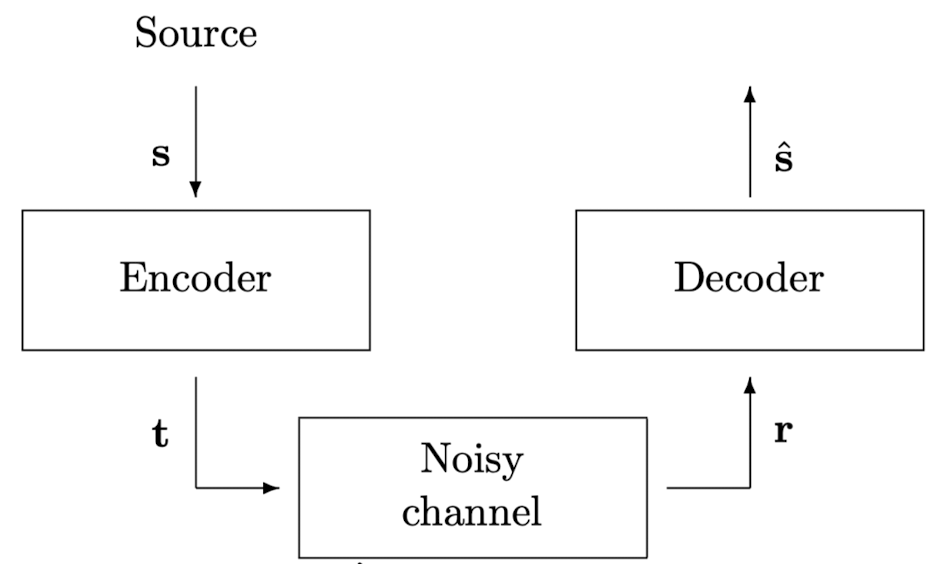
\includegraphics[width=0.5\linewidth]{images/BasicModel.jpg}
  \caption{Communication system model}
\end{figure}
In the digital communication system model, the source message $\mathbf{s}$ is encoded by an encoder into transmitted message $\mathbf{t}$, adding redundancy to the original message in some way. The channel is noisy, so it adds noise $\mathbf{n}$ to $\mathbf{t}$, yielding a received message $\mathbf{r}$. The decoder used the known redundancy introduced by the encoder to deduce the source message and the noise added.

\textbf{Information theory} is concerned with the theoretical limitations and potentials of such systems: What is the best error-correcting performance we could achieve? \textbf{Coding theory} is concerned with the creation of practical encoding and decoding systems.

\clearpage
\section{Probability, Entropy, and Inference}
\subsection{Probabilities and Ensembles}
\textbf{An ensemble $X$} is a triple $(x,\mathcal{A}_X,\mathcal{P}_X)$, where the \emph{outcome} $x$ is the value
of a random variable, which takes on one of a set of possible values,
$\mathcal{A}_X = \{a_1, a_2, \ldots, a_i, \ldots, a_I\}$, having probabilities
$\mathcal{P}_X = \{p_1, p_2, \ldots, p_I\}$,
with $P(x = a_i) = p_i$, $p_i \ge 0$ and $\sum_{a_i\in\mathcal{A}_X} P(x = a_i) = 1$.
\par\medskip
\noindent \textbf{A joint ensemble $XY$} is an ensemble in which each outcome is an ordered pair $x,y$ with $x \in \mathcal{A}_X = \{a_1,\ldots,a_I\}$ and $y \in \mathcal{A}_Y = \{b_1,\ldots,b_J\}$. We call $P(x,y)$ or $P(x\cap y)$ the joint probability of $x$ and $y$. Commas are optional when writing ordered pairs, so $xy \Leftrightarrow x,y$. N.B. In a joint ensemble $XY$ the two variables are not necessarily independent.

\par\medskip
\noindent \textbf{Marginal probability.} We can obtain the marginal probability $P(x)$ from the joint probability $P(x,y)$ by summation:
\begin{equation*}
  P(x=a_i) \equiv \sum_{y\in\mathcal{A}_Y} P(x=a_i,y).
\end{equation*}
Similarly, using briefer notation, the marginal probability of $y$ is:
\begin{equation*}
  P(y) \equiv \sum_{x\in\mathcal{A}_X} P(x,y).
\end{equation*}

\par\medskip
\noindent \textbf{Conditional probability.}
\begin{equation*}
  P(x=a_i \mid y=b_j) \equiv \frac{P(x=a_i,y=b_j)}{P(y=b_j)} \quad \text{if $P(y=b_j)\neq 0$.}
\end{equation*}
\[
  \text{[If $P(y=b_j)=0$ then $P(x=a_i \mid y=b_j)$ is undefined.]}
\]

\par\medskip
\noindent \textbf{Product rule} -- obtained from the definition of conditional probability:
\begin{equation*}
  P(x,y) = P(x\mid y)P(y)
  = P(y\mid x)P(x).
\end{equation*}
Or,
\begin{equation*}
  P(x,y\mid \mathcal{H}) = P(x\mid y,\mathcal{H})P(y\mid \mathcal{H})
  = P(y\mid x,\mathcal{H})P(x\mid \mathcal{H}).
\end{equation*}
This rule is also known as the chain rule.

\par\medskip
\noindent \textbf{Sum rule} -- a rewriting of the marginal probability definition:
\begin{equation*}
  P(x) = \sum_{y} P(x,y)
  = \sum_{y} P(x\mid y)P(y).
\end{equation*}
Or,
\begin{equation*}
  P(x\mid \mathcal{H}) = \sum_{y} P(x,y\mid \mathcal{H})
  = \sum_{y} P(x\mid y,\mathcal{H})P(y\mid \mathcal{H}).
\end{equation*}

\par\medskip
\noindent \textbf{Bayes' theorem} -- obtained from the product rule:
\begin{equation*}
  P(y\mid x) = \frac{P(x\mid y)P(y)}{P(x)}
  = \frac{P(x\mid y)P(y)}{\sum_{y'} P(x\mid y')P(y')}.
\end{equation*}
Or,
\begin{equation*}
  P(y\mid x,\mathcal{H}) = \frac{P(x\mid y,\mathcal{H})P(y\mid \mathcal{H})}{P(x\mid \mathcal{H})}
  = \frac{P(x\mid y,\mathcal{H})P(y\mid \mathcal{H})}{\sum_{y'} P(x\mid y',\mathcal{H})P(y'\mid \mathcal{H})}.
\end{equation*}
Bayes' theorem for continuous random variables replaces probabilities with probability density functions, and using integrations instead of summations.

\par\medskip
\noindent \textbf{Independence.} Two random variables $X$ and $Y$ are \emph{independent} (sometimes written $X\perp Y$) if and only if
\begin{equation*}
  P(x,y) = P(x)P(y).
\end{equation*}

\subsection{Forward Probabilities and Inverse Probabilities}

\textbf{Forward probability} problems involve a generative model that describes a process that is assumed to give rise to some data; the task is to compute the probability distribution or expectation of some quantity that depends on the data. 

\noindent \textbf{Inverse probability} problems involve a generative model of a process, but instead of computing the probability distribution of some quantity produced by the process, we compute the conditional probability of one or more of the unobserved variables in the process, given the observed variables. This invariably requires the use of Bayes' theorem.

\par\medskip
If $\theta$ denotes the unknown parameters, $D$ denotes the data, and $\mathcal{H}$ denotes the overall hypothesis space, the general equation:
\begin{equation*}
  P(\theta \mid D,\mathcal{H}) = \frac{P(D\mid \theta,\mathcal{H})P(\theta\mid \mathcal{H})}{P(D\mid \mathcal{H})}.
\end{equation*}
is written:
\begin{equation*}
  \text{posterior} = \frac{\text{likelihood}\times \text{prior}}{\text{evidence}}.
\end{equation*}
\noindent note that $P(\theta \mid D,\mathcal{H})$ is called the posterior probability of $\theta$ given $D$, $P(\theta\mid \mathcal{H})$ is called the prior probability of $\theta$, $P(D\mid \mathcal{H})$ is called the evidence or marginal likelihood. 

It is worth noticing that $P(D\mid \theta,\mathcal{H})$ is called the likelihood of $\theta$. The term likelihood and probability are not synonyms. The quantity $P(D\mid \theta,\mathcal{H})$ is a function of both $\theta$ and $D$: for fixed $D$, it defines the likelihood of $\theta$; for fixed $\theta$, it defines the probability over $D$.

This leads to \textbf{the likelihood principle}.

\begin{theorem}[Likelihood Principle]
Given a generative model for data $D$ given parameters $\theta$, $P(D\mid \theta)$, and having observed a particular outcome $d_1$, all inferences and predictions should depend only on the function $P(D_1\mid \theta)$.
\end{theorem}

An example which illustrates this idea well is as follows. Urn A contains three balls: one black, and two white; urn B contains three balls: two black, and one white. One of the urns is selected at random and one ball is drawn. The ball is black. What is the probability that the selected urn is urn A? 
\[
    P(A \mid \mathtt{black}) = \frac{P(\mathtt{black}\mid A)P(A)}{P(\mathtt{black}\mid A)+P(\mathtt{black}\mid B)} = \frac{\frac{1}{3}\times \frac{1}{2}}{\frac{1}{3} + \frac{2}{3}} = \frac{1}{6}
\]
Second scenario is similar. Urn A contains five balls: one black, two white, one green and one pink; urn B contains five hundred balls: 200 black, 100 white, 50 yellow, 40 cyan, 30 sienna, 25 green, 25 silver, 20 gold, and 10 purple. One of the urns is selected at random and one ball is drawn. The ball is black. What is the probability that the urn is urn A?
\[
    P(A \mid \mathtt{black}) = \frac{P(\mathtt{black}\mid A)P(A)}{P(\mathtt{black}\mid A)+P(\mathtt{black}\mid B)} = \frac{\frac{1}{5}\times \frac{1}{2}}{\frac{1}{5} + \frac{2}{5}} = \frac{1}{6}
\]
The details of the other possible outcomes and their probabilities are irrelevant. All that matters is the probability of the outcomes that actually happened (eg. the ball drawn was black) given the different hypotheses.

\subsection{Inference using Bayes' Theorem}

The first inference problem.
\begin{quote}
Unstable particles are emitted from a source and decay at a distance $x$, a real number that has an exponential probability distribution with characteristic length $\lambda$. Decay events can be observed only if they occur in a window extending from $x=1\,\mathrm{cm}$ to $x=20\,\mathrm{cm}$. $N$ decays are observed at locations $\{x_1,\ldots,x_N\}$. What is $\lambda$?
\end{quote}

Consider the probability of one data point, given $\lambda$:
\begin{equation*}
  P(x\mid \lambda)=
  \begin{cases}
    \dfrac{1}{\lambda}e^{-x/\lambda}/Z(\lambda) & 1<x<20,\\[4pt]
    0 & \text{otherwise.}
  \end{cases}
\end{equation*}
where the normalising constant makes the total probability is 1,
\begin{equation*}
  Z(\lambda)=\int_{1}^{20}\!dx\,\frac{1}{\lambda}e^{-x/\lambda}
  = \left(e^{-1/\lambda}-e^{-20/\lambda}\right).
\end{equation*}
Then introduce the Bayes' theorem:
\begin{align*}
  P\!\left(\lambda \mid \{x_1,\ldots,x_N\}\right)
  &= \frac{P(\{x\}\mid \lambda)\,P(\lambda)}{P(\{x\})}\\
  &\propto \frac{1}{\left(\lambda Z(\lambda)\right)^N}\exp\!\left(-\sum_{n=1}^{N}x_n/\lambda\right)P(\lambda).
\end{align*}

\begin{figure}[H]
    \begin{subfigure}{0.45\textwidth}
    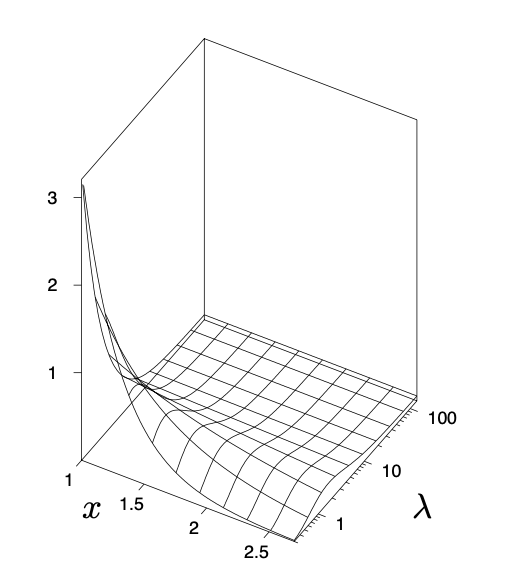
\includegraphics[width=0.9\linewidth]{images/DistributionInference.jpg}
    \caption{$P(x\mid \lambda)$ as a function of $x$ and $\lambda$. If $x$ is fixed, then it is the likelihood function of $\lambda$.}
    \end{subfigure}
    \hfill
    \begin{subfigure}{0.45\textwidth}
    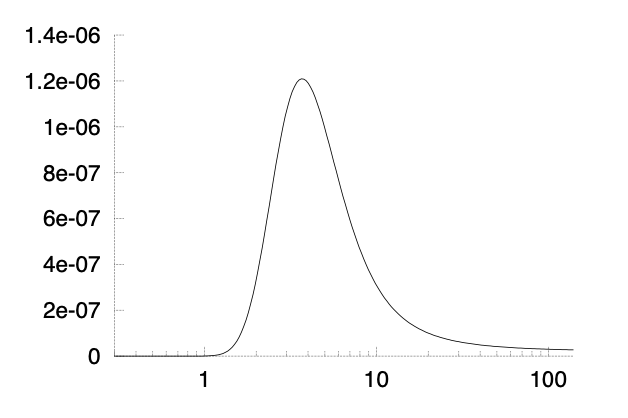
\includegraphics[width=0.9\linewidth]{images/SampleInference.jpg}
    \caption{the likelihood function in the case of $P(\{x\}=\{1.5, 2, 3, 4, 5, 12\}\mid \lambda)$ as a function of $\lambda$, which is the product of 6 likelihood functions for every element in $\{x\}$.}
    \end{subfigure}
\end{figure}

Probability are used here to quantify degrees of belief given assumptions (here, $P(\lambda)$ is the assumption).Once assumptions are made, the inferences are objective and unique, reproducible with complete agreement by anyone who has the same information and makes the same assumptions. Also, Bayesian uses a probability distribution P does not mean that he thinks of the world as stochastically changing its nature between the states described by the different hypotheses. He uses the notation of probabilities to represent his beliefs about the mutually exclusive micro-hypotheses (here, values of $\lambda$), of which only one is actually true.

\subsection{Entropy and Related Functions}
The \textbf{Shannon information content},
  \[
    h(x) \equiv \log_2 \frac{1}{P(x)}
  \]
is a measure of the information content of the outcome $x=a_i$, and it measures the length of the binary file that encodes the outcome. The \textbf{marginal entropy} of the ensemble,
  \[
    H(X) = \sum_i P(x)\log_2 \frac{1}{P(x)}
  \]
\noindent is the expected value of the Shannon information content for an ensemble $X$. They are all measured in bits, and another name for entropy of $X$ is the uncertainty of $X$. Some property of the entropy are
\begin{itemize}
  \item $H(X) \geq 0$ with equality iff $p_i = 1$ for one $i$, i.e. the outcome is certain
  \item entropy is maximised is $\mathbf{p}$ is uniform: $H(X) \leq \log_2 (|\mathcal{A}_X|)$ with equality iff $p_i = 1/|\mathcal{A}_X|$ for all $i$
\end{itemize}

The \textbf{joint entropy} of $X$ and $Y$
\[
  H(X,Y) = \sum_{xy \in \mathcal{A}_X \mathcal{A}_Y} P(x,y)\log \frac{1}{P(x,y)}.
\]
the entropy is additive for independent random variables: $H(X,Y) = H(X) + H(Y)$ iff $P(x,y)=P(x)P(y)$.

The \textbf{relative entropy} or Kullback-Leibler divergence between two probability distributions $P(x)$ and $Q(x)$ that are defined over the same
alphabet $\mathcal{A}_X$ is
\[
  D_{\mathrm{KL}}(P\|Q) = \sum_x P(x)\log \frac{P(x)}{Q(x)}.
\]
note that $D_{\mathrm{KL}}(P\|Q)\neq D_{\mathrm{KL}}(Q\|P)$. The relative entropy satisfies \textbf{Gibbs' inequality},
\[
  D_{\mathrm{KL}}(P\|Q) \ge 0
\]
with equality only if $P(x) = Q(x)$. Expanding the relative entropy, it gives $D_{\mathrm{KL}}(P\|Q) = \sum_x P(x)\log P(x) - \sum_x P(x) \log Q(x) = -H(p) + H(p,q)$, where $H(p)$ is an alternative way of writing $H(X)$ if $X \sim p$ and $H(p,q) = -\sum_x P(x) \log Q(x) = E_{X \sim p}[-\log_2 Q(x)]$ is called \textbf{cross entropy}. Since the relative entropy is always greater than or equals to zero, then $H(p,q) \geq H(p)$. An important intuition behind this is:
\begin{itemize}
  \item the Shannon information content $h(x = a_i)$ denotes the bits required to encode that specific outcome $a_i$
  \item $H(p)$ or $H(X)$, expected value of the Shannon information content, is the average number of bits required to encode one outcome from $X \sim p$
  \item $H(p,q)$ is the average number of bits required to encode one outcome from $X \sim p$, but by assuming $X$ is drawn from a different distribution $q$
  \item with a wrong model, bits will be wasted on average
\end{itemize}

\textbf{The conditional entropy of $X$ given $y=b_k$} is the entropy of the
probability distribution $P(x\mid y=b_k)$.
\[
  H(X\mid y=b_k) \equiv \sum_{x\in\mathcal{A}_X} P(x\mid y=b_k)\log \frac{1}{P(x\mid y=b_k)}.
\]

\textbf{The conditional entropy of $X$ given $Y$} is the average, over $y$, of
the conditional entropy of $X$ given $y$.
\begin{align*}
  H(X\mid Y)
  &\equiv \sum_{y\in\mathcal{A}_Y} P(y)
  \left[\sum_{x\in\mathcal{A}_X} P(x\mid y)\log \frac{1}{P(x\mid y)}\right]\\
  &= \sum_{xy\in\mathcal{A}_X\mathcal{A}_Y} P(x,y)\log \frac{1}{P(x\mid y)}.
\end{align*}
This measures the average uncertainty (i.e. expectation of $H(X\mid y)$) that remains about $x$ when $y$ is known. $H(X\mid Y) \leq H(X)$ means that additional information always reduce uncertainties, or at least no increase.

\textbf{Chain rule for information content.} From the product rule for
probabilities, we obtain:
\[
  \log \frac{1}{P(x,y)} = \log \frac{1}{P(x)} + \log \frac{1}{P(y\mid x)}
\]
so
\[
  h(x,y) = h(x) + h(y\mid x).
\]
In words, this says that the information content of $x$ and $y$ is the
information content of $x$ plus the information content of $y$ given $x$.

\textbf{Chain rule for entropy.} The joint entropy, conditional entropy and
marginal entropy are related by:
\[
  H(X,Y) = H(X) + H(Y\mid X) = H(Y) + H(X\mid Y).
\]
In words, this says that the uncertainty of $X$ and $Y$ is the uncertainty of
$X$ plus the uncertainty of $Y$ given $X$.

\textbf{The mutual information between $X$ and $Y$} is
\[
  \begin{aligned}
  I(X;Y) &\equiv H(X) - H(X\mid Y) \\
  &= \sum_x P(x) \log \frac{1}{P(x)} - \sum_{xy} P(x,y) \log \frac{1}{P(x \mid y)} \\
  &= \sum_{xy} P(x) P(y \mid x) \log \frac{1}{P(x)} - \sum_{xy} P(x,y) \log \frac{1}{P(x \mid y)} \\
  &= \sum_{xy} P(x,y) \log \frac{P(x,y)}{P(x) P(y)}
  \end{aligned}
\]
and satisfies $I(X;Y)=I(Y;X)$, and $I(X;Y)\geq 0$. It measures the average
reduction in uncertainty about $x$ that results from learning the value of $y$;
or vice versa, the average amount of information that $x$ conveys about $y$.

\textbf{The conditional mutual information between $X$ and $Y$ given $z=c_k$}
is the mutual information between the random variables $X$ and $Y$ in the joint
ensemble $P(x,y\mid z=c_k)$,
\[
  I(X;Y\mid z=c_k) = H(X\mid z=c_k) - H(X\mid Y,z=c_k).
\]

\textbf{The conditional mutual information between $X$ and $Y$ given $Z$} is
the average over $z$ of the above conditional mutual information.
\[
  I(X;Y\mid Z) = H(X\mid Z) - H(X\mid Y,Z).
\]
No other ``three-term entropies'' will be defined. For example, expressions such
as $I(X;Y;Z)$ and $I(X\mid Y;Z)$ are illegal. But you may put conjunctions of
arbitrary numbers of variables in each of the three spots in the expression
$I(X;Y\mid Z)$ - for example, $I(A,B;C,D\mid E,F)$ is fine: it measures how much
information on average $c$ and $d$ convey about $a$ and $b$, assuming $e$ and
$f$ are known.

\textbf{Chain rule for mutual information}:
\[
  I(X;Y,Z) = I(X;Y) + I(X;Z\mid Y).
\]

\begin{figure}[H]
  \centering
  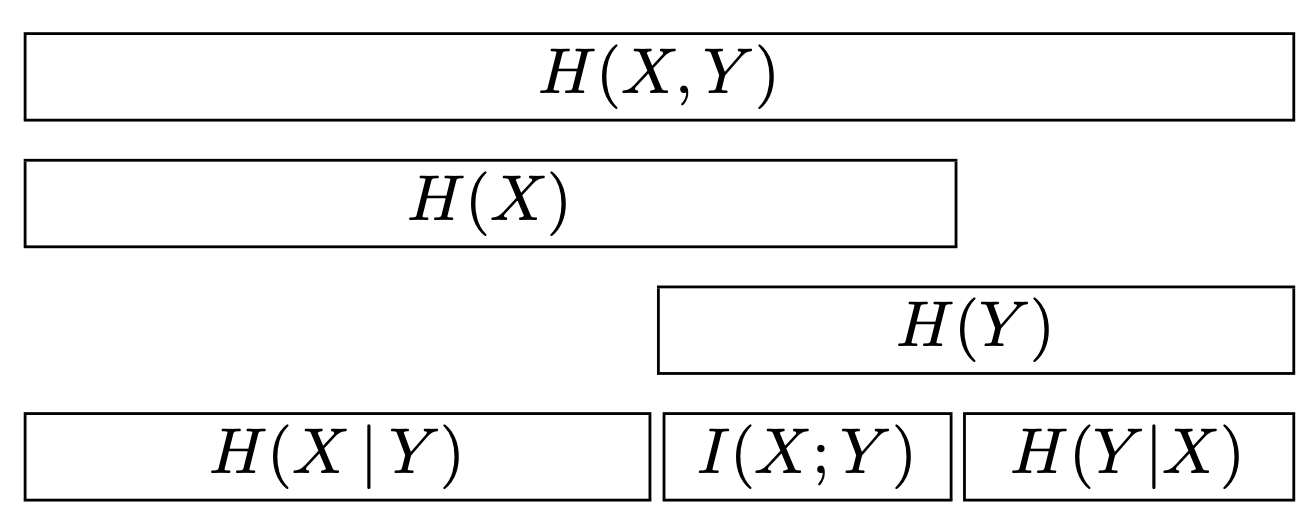
\includegraphics[width=0.5\linewidth]{images/MutualInfo.png}
  \caption{Relationship between joint information, marginal entropy, conditional entropy and mutual entropy}
\end{figure}


\subsection{Data Processing Theorem}

The data processing theorem states that data processing can only destroy information. 

Considering an ensemble $WDR$ in which $w$ be the state of the world, $d$ be the data gathered, and $r$ be the
processed data, so that these three variables form a Markov chain
\[
  w \to d \to r,
\]
that is, the probability $P(w,d,r)$ can be written as
\[
  P(w,d,r) = P(w)P(d\mid w)P(r\mid d).
\]
An important observation from this: 
\[
  P(w\mid d,r) = \frac{P(w,d,r)}{P(d,r)} = \frac{P(w)P(d\mid w)P(r\mid d)}{P(d,r)}=\frac{P(w\mid d)P(d)P(r\mid d)}{P(d,r)} = P(w\mid d)
\]
Therefore, $I(W;R\mid D) = H(W\mid D) - H(W\mid D,R) = 0$, which means there will be no more information about $w$ once we know $d$.

Now, in the case $w \to d \to r$, $w$ and $r$ are independent given $d$, so
$I(W;R\mid D)=0$. Using the chain rule twice, we have:
\[
  I(W;D,R) = I(W;D) + I(W;R\mid D) = I(W;D)
\]
and
\[
  I(W;D,R) = I(W;R) + I(W;D\mid R),
\]
so
\[
  I(W;R) \leq I(W;D).
\]
The average information that $R$ conveys about $W$, $I(W;R)$, is less
than or equal to the average information that $D$ conveys about $W$, $I(W;D)$.

\clearpage
\section{The Source Coding Theorem}

\textbf{An ensemble $X$} is a triple $(x,\mathcal{A}_X,\mathcal{P}_X)$, where the \emph{outcome} $x$ is the value
of a random variable, which takes on one of a set of possible values,
$\mathcal{A}_X = \{a_1, a_2, \ldots, a_i, \ldots, a_I\}$, having probabilities
$\mathcal{P}_X = \{p_1, p_2, \ldots, p_I\}$,
with $P(x = a_i) = p_i$, $p_i \ge 0$ and $\sum_{a_i\in\mathcal{A}_X} P(x = a_i) = 1$.

Measures of the information content of an outcome $x=a_i$ from such an ensemble follows these assertions:

\begin{enumerate}
  \item the \emph{Shannon information content},
  \[
    h(x=a_i) \equiv \log_2 \frac{1}{p_i},
  \]
  is a measure of the information content of the outcome $x=a_i$, and it measures the length of the binary file that encodes the outcome.

  \item the \emph{entropy} of the ensemble,
  \[
    H(X) = \sum_i p_i\,\log_2 \frac{1}{p_i},
  \]
  \noindent is a measure of the information content of the ensemble.
\end{enumerate}
\begin{figure}[H]
    \begin{subfigure}{0.45\textwidth}
    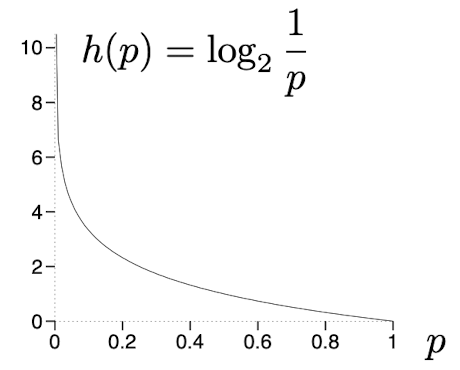
\includegraphics[width=0.9\linewidth]{images/h_p.jpg}
    \caption{the Shannon information content of an outcome with probability p, as a function of p. The less probable an outcome is, the greater its Shannon information content.}
    \end{subfigure}
    \hfill
    \begin{subfigure}{0.45\textwidth}
    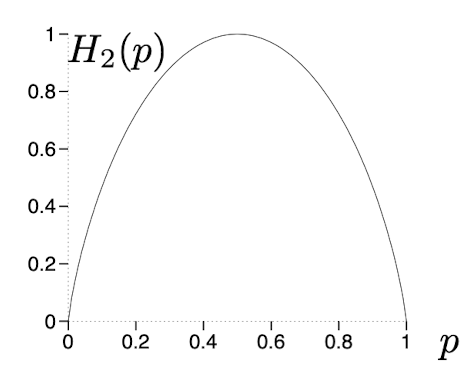
\includegraphics[width=0.9\linewidth]{images/H2_p.jpg}
    \caption{the binary entropy function, $H_2(X)=p \log_2\frac{1}{p} + (1-p)\log_2\frac{1}{1-p}$, which is the entropy of the ensemble $X$ whose alphabet and probability distribution are $\mathcal{A}_X=\{a,b\},\,\mathcal{P}_X=\{p,(1-p)\}$.}
    \end{subfigure}
\end{figure}

The \textbf{definition of independence} is that the probability distribution is separable into a product:
\[
  P(x,y) = P(x)P(y)
\]
Also, the information gained also have the property of additivity, such that the Shannon information content of the outcomes x, y is
\[
  h(x,y) = h(x)+h(y),\quad \text{if $X$ and $Y$ are independent.}
\]
additivty applies also for the entropy
\[
  H(X,Y) = H(X)+H(Y),\quad \text{if $X$ and $Y$ are independent.}
\]
Therefore, if there are $N$ independent and identically distributed random variables $X$, the entropy of $X^N$ is therefore $H(X^N) = NH(X)$, where $(X_1,X_2,...,X_N)$ is denoted by $X^N$.
\subsection{Lossless Compression}
One way of measuring the information content of a random variable is simply to count the number of possible outcomes, $|\mathcal{A}_X|$. If we gave a binary name to each outcome, the length of each name would be $\log_2|\mathcal{A}_X|$.

\textbf{The raw bit content} of $X$ is
\[
  H_0(X) = \log_2 |\mathcal{A}_X|.
\]
$H_0(X)$ is a lower bound for the number of binary questions that are always guaranteed to identify an outcome from the ensemble $X$. It is an additive quantity: the raw bit content of an ordered pair $x,y$, having $|\mathcal{A}_X||\mathcal{A}_Y|$ possible outcomes, satisfies
\[
  H_0(X,Y) = H_0(X) + H_0(Y).
\]

This measure of information content does not include any probabilistic element, and the encoding rule it corresponds to does not compress the source data; it simply maps each outcome to a constant-length binary string. This is an example of a \textbf{lossless compressor} which maps all the files to different encodings.

\subsection{Lossy Compression}
A \textbf{lossy compressor} compresses some files, but maps some files to the same encoding. Assuming that the user requires perfect recovery of the source file, so the occurrence of one of these confusable files leads to a failure. Denoting the probability that the source string is one of the confusable files by $\delta$, so \textbf{a lossy compressor has a probability $\delta$ of failure}. If $\delta$ can be made very small then a lossy compressor may be practically useful.

\subsubsection{The Smallest $\delta$-Sufficient Subset}
The smallest $\delta$-sufficient subset $S_\delta$ is the smallest subset of $\mathcal{A}_X$ satisfying
\[
  P(x \in S_\delta) \geq 1-\delta
\]
The subset $S_\delta$ can be constructed by ranking the elements of $\mathcal{A}_X$ in order of decreasing probability and adding successive elements starting from the most probable elements until the total probability is $\geq (1-\delta)$.

This compression scheme motivates the following measure of information content:

\noindent \textbf{The essential bit content} of X is:
\[
  H_\delta(X) = \log_2(|S_\delta|)
\]
which can be interpreted as the number of bits required to encode every elements in $S_\delta$.

\subsubsection{The Source Coding Theorem and Typical Set}
How to compress blocks of symbols from a source? Consider an outcome $\mathbf{x} = (x_1,x_2,...,x_N)$ is a string of $N$ independent identically distributed random variables from a single ensemble $X$. Remember, its entropy $H(X^N) = NH(X)$.

Without any compression, there are $2^N$ possible outcomes $\mathbf{x}$, and for each of them $N$ bits are required to encode. In the limiting case where $N$ becomes very large, by selecting $2^{NH(X)}$ possible outcomes out of $2^N$ into the "typical set", it is possible to use $NH(X)$ bits in minimum to encode each outcomes. Additionally, those $2^{NH(X)}$ outcomes in the limiting case are equiprobable (probability concentrates in the typical set), each with a probability around $2^{-NH(X)}$.

This is formally described in \textbf{Shannon's source coding theorem},
\begin{theorem}[Shannon's source coding theorem]
Let $X$ be an ensemble with entropy $H(X)=H$ bits. Given $\epsilon>0$ and $0<\delta<1$, there exists a positive integer $N_0$ such that for $N>N_0$,
\[
  \left|\frac{1}{N}H_\delta\left(X^N\right)-H\right|<\epsilon.
\]
\end{theorem}
\noindent where the term $\frac{1}{N}H_\delta\left(X^N\right)$ is the average bits used per symbol after compression, and $H_\delta\left(X^N\right)$ can be calculated via $\log_2(\text{number of element in typical set})$. 

The theorem can be interpreted as \textbf{N i.i.d. random variables each with entropy $H(X)$ can be compressed into more than $NH(X)$ bits with negligible risk of information loss, as $N \to \infty$; conversely if they are compressed into fewer than $NH(X)$ bits it is virtually certain that information will be lost}. Therefore, with this theorem, we can define an algorithm that gives a distinct name of length $NH(X)$ bits to each $\mathbf{x}$ in the typical set.

Let us define typicality for an arbitrary ensemble $X$ with alphabet $\mathcal{A}_X$. Our definition of a \textbf{typical string} will involve the string's probability. \textbf{A long string of $N$ symbols will usually contain about $p_1N$ occurrences of the first symbol, $p_2N$ occurrences of the second, etc}. Hence the probability of this string is roughly
\[
  P(\mathbf{x})_{\mathrm{typ}} = P(x_1)P(x_2)P(x_3)\cdots P(x_N) \simeq p_1^{(p_1N)}\,p_2^{(p_2N)}\,\cdots\,p_I^{(p_IN)}.
\]
so that the information content of a typical string is
\[
  \log_2\frac{1}{P(\mathbf{x})} \simeq N\sum_i p_i\,\log_2\frac{1}{p_i} = NH.
\]
So the random variable $\log_2\frac{1}{P(\mathbf{x})}$, which is the information content of $\mathbf{x}$, is very likely to be close in value to $NH$. The definition of typicality is built on this observation.

We define the typical elements of $\mathcal{A}_X^N$ to be those elements that have probability close to $2^{-NH}$. (Note that the typical set, unlike the smallest sufficient subset, does not include the most probable elements of $\mathcal{A}_X^N$, but it can be shown that these most probable elements contribute negligible probability.)

A parameter $\beta$ is introduced that defines how close the probability has to be to $2^{-NH}$ for an element to be "typical". We call the set of typical elements the typical set, $T_{N\beta}$:
\[
  T_{N\beta} \equiv \left\{\mathbf{x}\in \mathcal{A}_X^N : \left|\frac{1}{N}\log_2\frac{1}{P(\mathbf{x})} - H\right| < \beta\right\}.
\]

It can be shown that whatever value of $\beta$ is chosen, the typical set contains almost all the probability as $N$ increases. The elements are similar in probability only in the sense that their values of $\log_2(\frac{1}{P(\mathbf{x})})$ are within $2N\beta$ of each other. This result is summarised by the \textbf{asymptotic equipartition principle}.

\begin{theorem}[Asymptotic equipartition principle]
  For an ensemble of $N$ independent identically distributed (i.i.d.) random variables $X^N\equiv (X_1,X_2,\ldots,X_N)$, with $N$ sufficiently large, the outcome $\mathbf{x}=(x_1,x_2,\ldots,x_N)$ is almost certain to belong to a subset of $\mathcal{A}_X^N$, having only $2^{NH(X)}$ members, each having probability close to $2^{-NH(X)}$.
\end{theorem}

Notice that if $H(X) < H_0(X)$ then $2^{NH(X)}$ is a tiny fraction of the number of possible outcomes $|\mathcal{A}_X^N| = |\mathcal{A}_X|^N = 2^{NH_0(X)}$.

\begin{figure}[H]
  \centering
  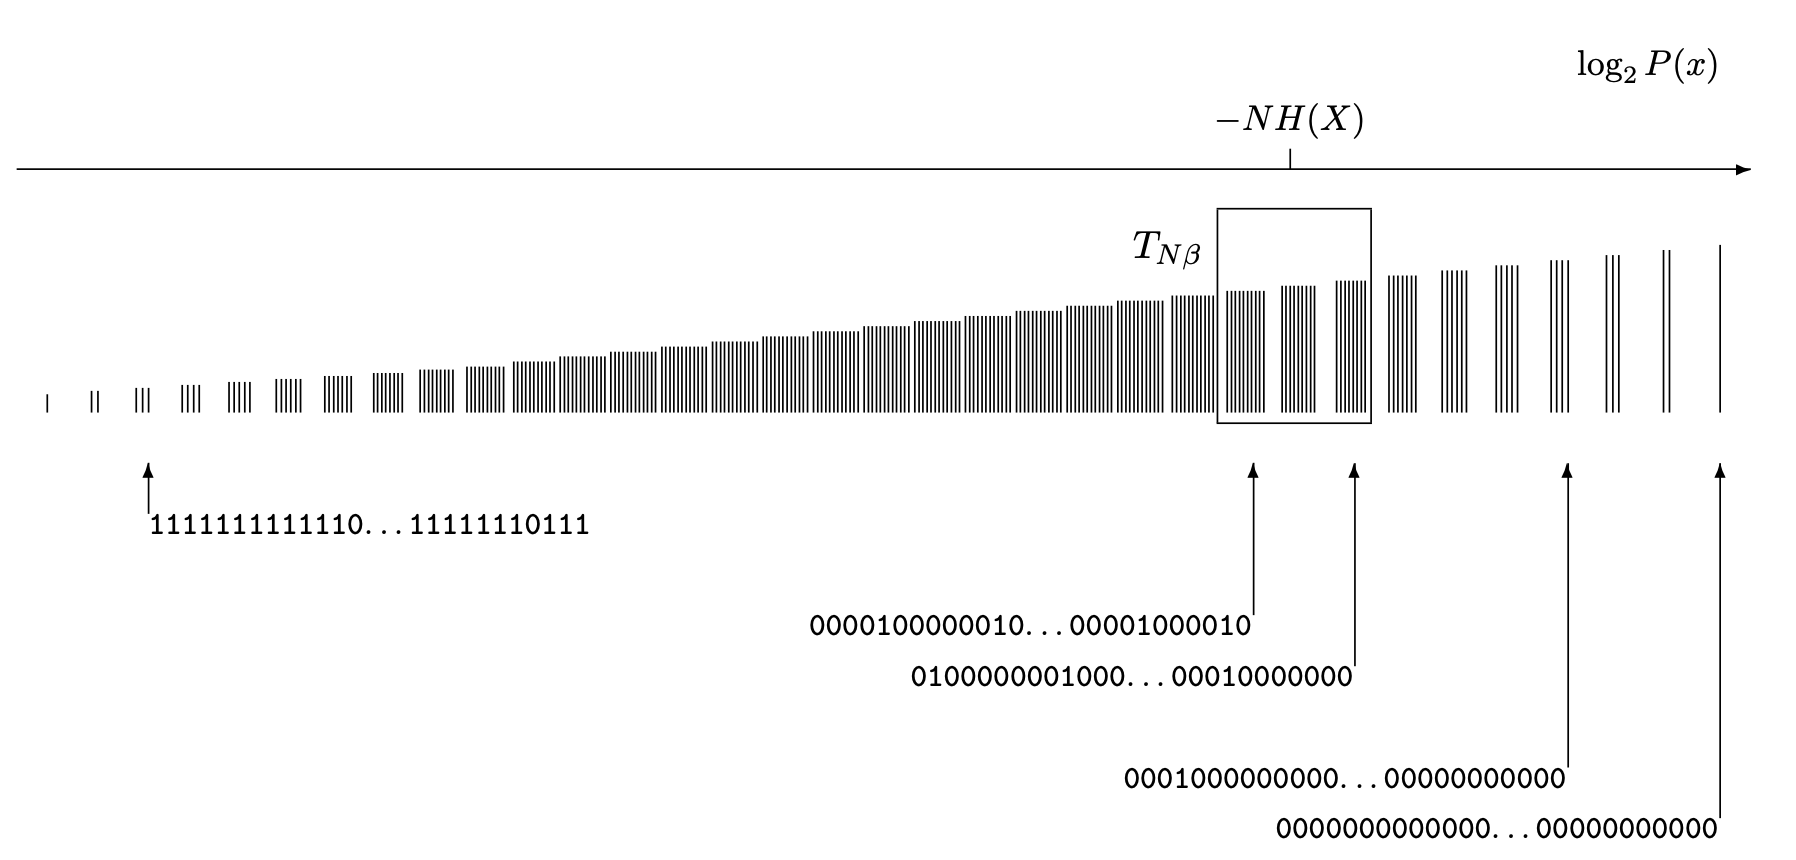
\includegraphics[width=0.9\linewidth]{images/typical_set.jpg}
  \caption{Schematic diagram showing all strings in the ensemble $X^N$ ranked by their probability, and the typical set $T_{N\beta}$}
\end{figure}

\subsection{Comments on Source Coding Theorem}
\begin{enumerate}
  \item The source coding theorem has two parts, $\frac{1}{N}H_\delta(X^N) < H+\epsilon$, and $\frac{1}{N}H_\delta(X^N) > H-\epsilon$. Part 1 tells that even if the probability of error $\delta$ is extremely small, the number of bits per symbol $\frac{1}{N}H_\delta(X^N)$ needed to specify a long $N$-symbol string $\mathbf{x}$ with vanishingly small error probability does not have to exceed $H+\epsilon$ bits. We need to have only a tiny tolerance for error, and the number of bits required drops significantly from $H_0(X)$ to $(H+\epsilon)$. Part 2 tells us that even if $\delta$ is very close to 1, so that errors are made most of the time, the average number of bits per symbol needed to specify $\mathbf{x}$ must still be at least $H-\epsilon$ bits. These two extremes tell us that \textbf{regardless of our specific allowance for error, the number of bits per symbol needed to specify $\mathbf{x}$ is $H$ bits; no more and no less}.
  \begin{figure}[H]
  \centering
  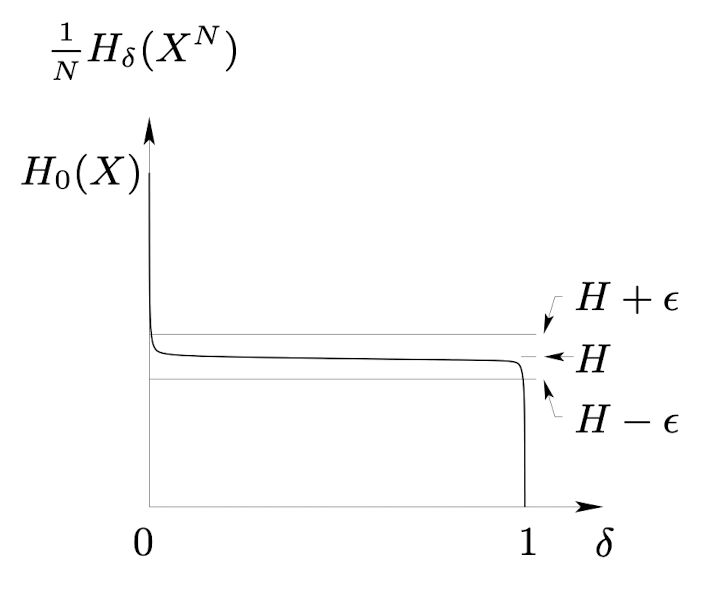
\includegraphics[width=0.4\linewidth]{images/sourcecoding.jpg}
  \caption{Schematic illustration of the two parts of the theorem. Given any $\delta$ and $\epsilon$, we show that for large enough $N$, $\frac{1}{N}H_\delta(X^N)$ lies (1) below the line $H + \epsilon$ and (2) above the line $H - \epsilon$.}
  \end{figure}
  \item The best choice of subset for block compression is (by definition) $S_\delta$, not a typical set. So why did we bother introducing the typical set? The answer is, we can count the typical set. We know that all its elements have ``almost identical'' probability ($2^{-NH}$), and we know the whole set has probability almost 1, so the typical set must have roughly $2^{NH}$ elements. Without the help of the typical set (which is very similar to $S_\delta$) it would have been hard to count how many elements there are in $S_\delta$.
\end{enumerate}

\clearpage
\section{The Channel Coding Theorem}
\begin{figure}[H]
  \centering
  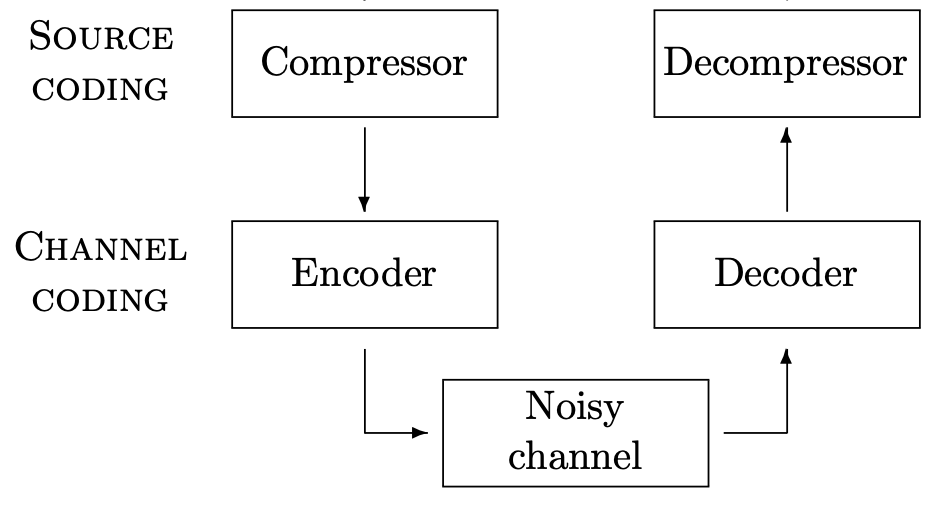
\includegraphics[width=0.6\linewidth]{images/ChannelBigPicture.png}
  \caption{Overview of source coding and channel coding}
\end{figure}

\subsection{Noisy Channel}

\textbf{A discrete memoryless channel $Q$} is characterized by an input alphabet
$\mathcal{A}_X$, an output alphabet $\mathcal{A}_Y$, and a set of conditional
probability distributions $P(y\mid x)$, one for each $x\in\mathcal{A}_X$. These transition probabilities may be written in a matrix
\[
  Q_{j\mid i} = P(y=b_j\mid x=a_i).
\]
Orienting this matrix with the output variable $j$ indexing the rows and
the input variable $i$ indexing the columns, so that each column of $\mathbf{Q}$
is a probability vector. With this convention, we can obtain the probability of
the output, $\mathbf{p}_Y$, from a probability distribution over the input,
$\mathbf{p}_X$, by right-multiplication:
\[
  \mathbf{p}_Y = \mathbf{Q}\mathbf{p}_X.
\]

\[
  \begin{bmatrix}
    P(y=b_1)\\
    \vdots\\
    P(y=b_j)
  \end{bmatrix}
  =
  \begin{bmatrix}
    P(y=b_1\mid x=a_1) & \cdots & P(y=b_1\mid x=a_i)\\
    \vdots & \ddots & \vdots\\
    P(y=b_j\mid x=a_1) & \cdots & P(y=b_j\mid x=a_i)
  \end{bmatrix}
  \begin{bmatrix}
    P(x=a_1)\\
    \vdots\\
    P(x=a_i)
  \end{bmatrix}.
\]

Channel $Q$ defines a set of conditional probabilities $P(y\mid x)$. If we define an input distribution $P(x)$, then we have a joint distribution $P(x,y) = P(y\mid x)P(x) $. Now if we receive a particular symbol $y$, what was the input symbol $x$? We won't know for certain, but we can write the posterior distribution of the input:
\[P(x\mid y) = \frac{P(y\mid x)P(x) }{P(y)} = \frac{P(y\mid x)P(x) }{\sum_{x^{\prime}} P(y\mid x^{\prime})P(x^{\prime})} \]

\textbf{The capacity} of a channel $Q$ is:
\[
  C(Q) = \max_{\mathcal{P}_X} I(X;Y).
\]
The distribution $\mathcal{P}_X$ that achieves the maximum is called the
\textbf{optimal input distribution}, denoted by $\mathcal{P}_X^{*}$. There may be
multiple optimal input distributions achieving the same value of $I(X;Y)$. We will tend to think of $I(X;Y)$ as $H(X)-H(X\mid Y)$, i.e., how much the uncertainty of the input $X$ is reduced when we look at the output $Y$. But for computational purposes it is often handy to evaluate $H(Y)-H(Y\mid X)$ instead.

\subsection{The Noisy-Channel Coding Theorem}

The theorem has three parts, two positive and one negative. The main positive
result is the first.

\begin{enumerate}
  \item For every discrete memoryless channel, the channel capacity
  \[
    C = \max_{\mathcal{P}_X} I(X;Y)
  \]
  has the following property. For any $\epsilon>0$ and $R<C$, for large enough
  $N$, there exists a code of length $N$ and rate $\geq R$ and a decoding
  algorithm, such that the maximal probability of block error is $<\epsilon$.

  \item If a probability of bit error $p_b$ is acceptable, rates up to $R(p_b)$
  are achievable, where
  \[
    R(p_b) = \frac{C}{1-H_2(p_b)}.
  \]

  \item For any $p_b$, rates greater than $R(p_b)$ are not achievable.
\end{enumerate}

\begin{figure}[H]
  \centering
  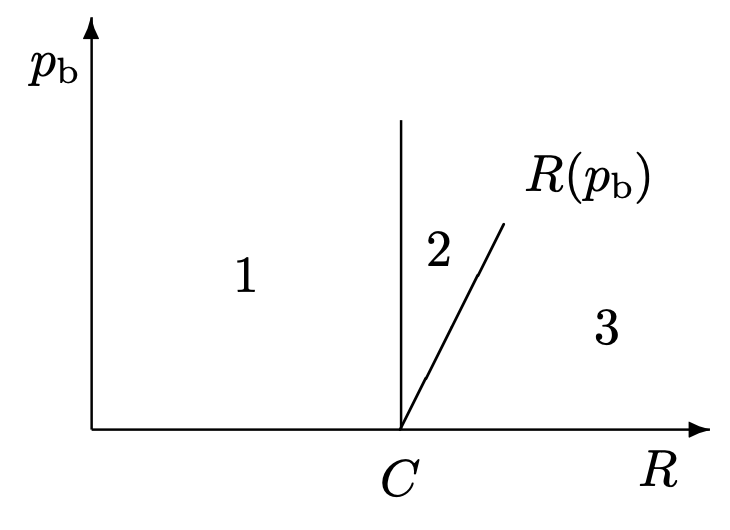
\includegraphics[width=0.5\linewidth]{images/NoisyChannelTheorem.png}
  \caption{Portion of the $R$, $p_b$ plane to be proved achievable (1,2) and not achievable (3)}
\end{figure}



\end{document}